%% TODO: Add a small paragraph to tell what this chapter is about
This chapter delves into ...

%% TODO: Make sure to use \textbf or \textit for highlighting keywords, and \cite{} to cite the corresponding quotations
\section{Current Advancements}
Integer at leo in libero facilisis pulvinar. Donec augue lorem, mattis eu sapien ut, maximus faucibus ex. Donec elementum vehicula lectus, ac laoreet quam condimentum in. Pellentesque id convallis arcu, facilisis posuere ligula. Sed in ante id nunc euismod lobortis. Nam dolor ex, faucibus vitae scelerisque vel, malesuada tempor ipsum. Integer lacinia pulvinar ex, ut accumsan nunc. Maecenas convallis felis velit, sed placerat quam faucibus a. Fusce odio urna, rhoncus et lorem nec, sollicitudin bibendum lorem. Donec eu bibendum quam. Nulla vel semper nisl, nec aliquet nulla. Vivamus fermentum leo justo, vel facilisis nisi bibendum sed. Sed at turpis risus. Praesent vestibulum tellus arcu, non aliquam elit aliquet eget. Praesent et lacinia massa.

\section{Research Gap}
Donec bibendum eget turpis tristique venenatis. Donec luctus justo non nunc sodales, ac vehicula elit fringilla. Cras vehicula, sem ut molestie hendrerit, ligula lectus ultricies nunc, eget vehicula turpis tortor pulvinar felis. Aliquam tempor mauris turpis, eget gravida ipsum dignissim non. Mauris et pretium ligula, eu auctor dolor. Curabitur risus justo, scelerisque vel sem quis, facilisis dictum ante. Cras pulvinar magna in erat ultricies scelerisque. In at laoreet mi, non sagittis elit. Duis id metus viverra, tristique purus in, laoreet leo.

%% TODO: Make sure to use \subsection{} and \subsubsection{} for smaller sections inside a larger sections
\section{Theoretical Background}
%% TODO: Use ~\ref{} to mention a labeled figure, table, section, or anything else
\subsection{Concept 1}
Sed eget lobortis leo. Maecenas ut tempor nibh. Nullam arcu nulla, aliquet vel enim maximus, gravida porta tortor. Orci varius natoque penatibus et magnis dis parturient montes, nascetur ridiculus mus. Donec aliquet luctus porttitor. Vivamus porta nulla ut tortor condimentum, at ullamcorper orci facilisis. Vivamus venenatis tellus vel dolor vestibulum, ac placerat orci laoreet. Praesent at elit arcu. Maecenas et lacus sit amet odio finibus semper. Mauris commodo vestibulum aliquam. Mauris non faucibus augue. Vivamus eleifend mauris eget mi venenatis, a maximus dolor mollis in Fig.~\ref{fig:1}.

%% TODO: Adjust the size of the figure by using [widht=.x\linewidth] (x is a fraction) to fit within the page width. Then rename to your picture file name, add the caption and a label
\begin{figure}[ht]
	\centering
	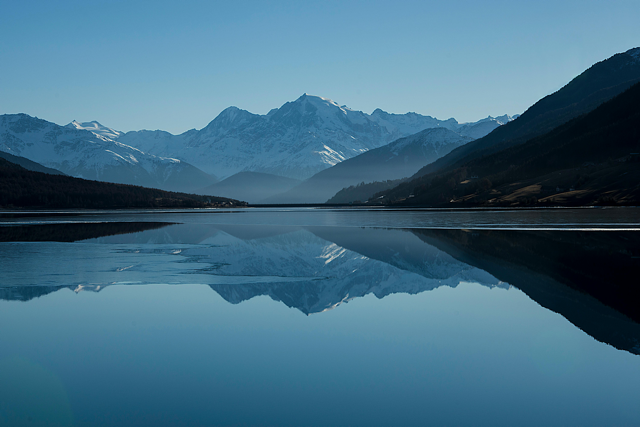
\includegraphics[width=\linewidth]{sample.png}
	\caption{The caption of the figure.}
	\label{fig:1}
\end{figure}

\subsubsection{More details of Concept 1}
Quisque sit amet ipsum sed ligula congue mattis viverra sit amet sem. Phasellus ante tortor, dictum id ex eget, lacinia pulvinar ligula. Aenean sodales in augue in tempus. Ut ut venenatis magna, feugiat tristique justo. Etiam ac mauris cursus, tincidunt elit commodo, molestie dolor. Nam maximus feugiat nunc, et facilisis eros malesuada vel. Suspendisse potenti. Cras ipsum eros, cursus vitae luctus ac, blandit pulvinar velit. Donec cursus viverra aliquet. Maecenas pharetra nec sem a gravida provided in Table~\ref{tab:1}.

\begin{table}[ht]
	\centering
	\caption{Comparison of different methods (\protect\cmark: YES, \protect\xmark: NO).}
	\label{tab:1}
	%% Comment the next line if the table width is relatively small
	\resizebox{\textwidth}{!}{%
		\begin{tabular}{lcccccc}
			\hline
			          & \textbf{Your Method} & Method B & Method C & Method D & Method E & Method F \\ \hline
			Feature 1 & \cmark               & \cmark   & \xmark   & \cmark   & \xmark   & \cmark   \\ 
			Feature 2 & \cmark               & \xmark   & \cmark   & \cmark   & \cmark   & \xmark   \\ 
			Feature 3 & \xmark               & \cmark   & \cmark   & \xmark   & \xmark   & \cmark   \\ 
		\end{tabular}%
		%%TODO: Also comment this } to match the above command
	}
\end{table}
	
	
%% TODO: For math mode, wrap the equation inside $ $ for inline mode, wrap inside $$ $$ for non-numbering block mode, or align environment as a numbered block equation
Ut consectetur quam in elit ullamcorper, non dictum velit congue. Nulla facilisi. Suspendisse potenti. Donec ut felis nec odio tempor rhoncus non a ex $\mathbb{G}_1$ where 

$$a \in \mathbb{G}_1$$

Aliquam efficitur fermentum metus, eu posuere orci commodo sit amet. Nullam vulputate consectetur sagittis. Donec imperdiet mi a facilisis facilisis. Cras at diam ornare, suscipit ipsum at, porta arcu. Orci varius natoque penatibus et magnis dis parturient montes, nascetur ridiculus mus. Mauris eu augue quis leo venenatis ultricies. Sed dapibus magna quam, ornare feugiat augue ullamcorper et.

\begin{align}
	e : \mathbb{G}_1 \times \mathbb{G}_2 & \rightarrow \mathbb{G}_T \\
	(a, b)                               & \mapsto e(a, b)          
\end{align}